\documentclass[a4paper,11pt]{article}
\usepackage[utf8]{inputenc}
\usepackage{graphicx}
\graphicspath{{immagini/}}
\usepackage{textcomp}
\usepackage{afterpage} 
\usepackage{afterpage} 
\usepackage{geometry}
\usepackage{booktabs}
\usepackage{amsmath}
\usepackage{amsfonts}
\usepackage{amssymb}
\usepackage{subfig}
\usepackage{geometry}
\usepackage{booktabs}
\usepackage{caption}
\usepackage{subfig}
\geometry{a4paper,top=3cm,bottom=3 cm,left=3.5cm,right=3.5cm,%
heightrounded,bindingoffset=5mm}
\usepackage{hyperref}
\newcommand{\HRule}{\rule{\linewidth}{0.5mm}}

\begin{document}
\begin{titlepage}
\begin{center}

% Upper part of the page. The '~' is needed because \\
% only works if a paragraph has started.
%\includegraphics[width=0.30\textwidth]{./immagini/logo.png}~\\[1cm]

\textsc{\LARGE Università degli studi di Padova}\\[1.5cm]

\textsc{\Large Physics Laboratory}\\[0.5cm]

% Title
\HRule \\[0.4cm]
{ \huge \bfseries Timing\\ [0.4cm] }

\HRule \\[1.5cm]

% Author and supervisor
\noindent
\begin{minipage}{0.4\textwidth}
\begin{flushleft} \large
\emph{Autori:}\\
Luca \textsc{Morselli}\\
Andrea \textsc{Raggio}\\
\end{flushleft}
\end{minipage}%
\begin{minipage}{0.4\textwidth}
\begin{flushright} \large
\emph{Docenti:} \\
Luca \textsc{stevanato}\\
Francesco \textsc{recchia}\\
\end{flushright}
\end{minipage}

\vfill

% Bottom of the page
{\large \today}

\end{center}
\end{titlepage}

\section*{Key points of the experiment}


\section*{Energy Calibration}


\begin{figure}[h!]
\centering
\subfloat[][\emph{Detector \#1 spectrum}.]
   {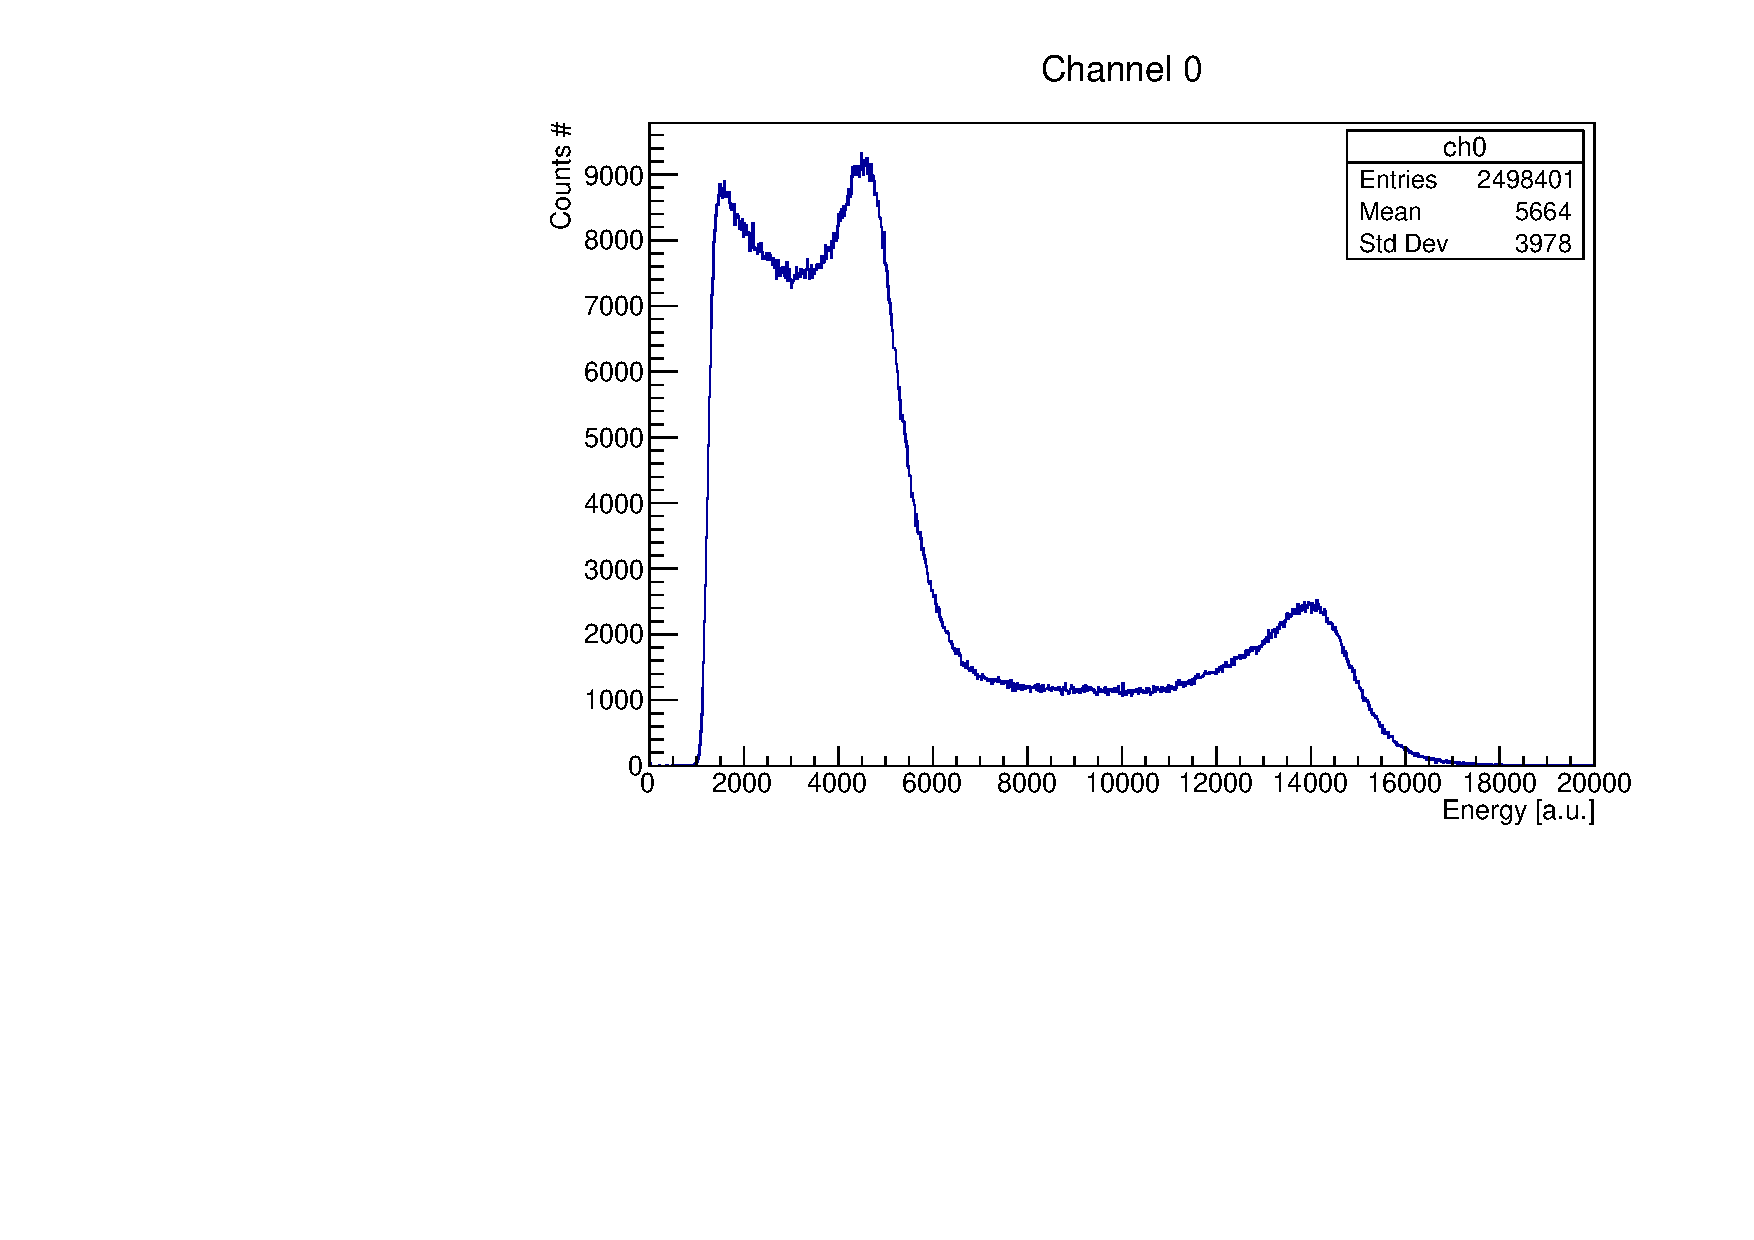
\includegraphics[width=.45\textwidth]{d1_spectrum_qlong}} \quad
\subfloat[][\emph{Detector \#2 spectrum}.]
   {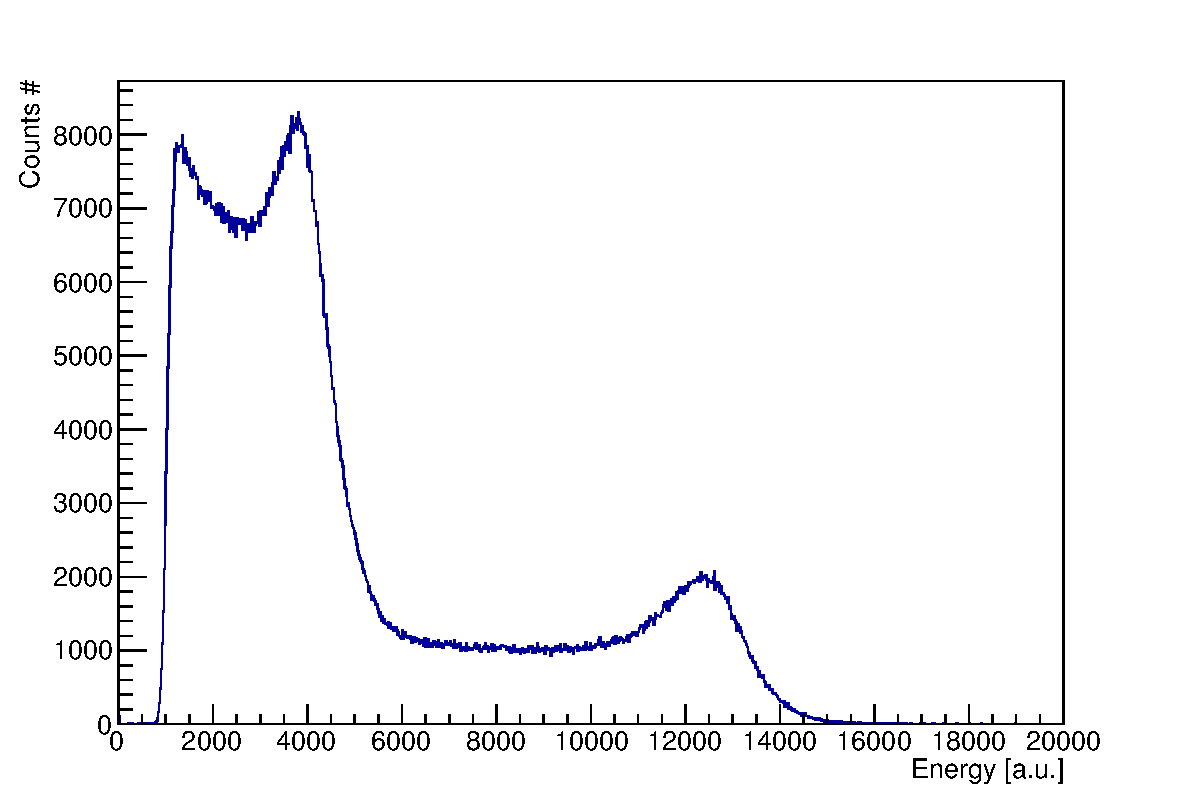
\includegraphics[width=.45\textwidth]{d2_spectrum_qlong}} \\
\caption{Detectors spectra (not calibrated).}
\end{figure}

\begin{figure}[h!]
\centering
\subfloat[][\emph{Low energy Compton Edge}.]
   {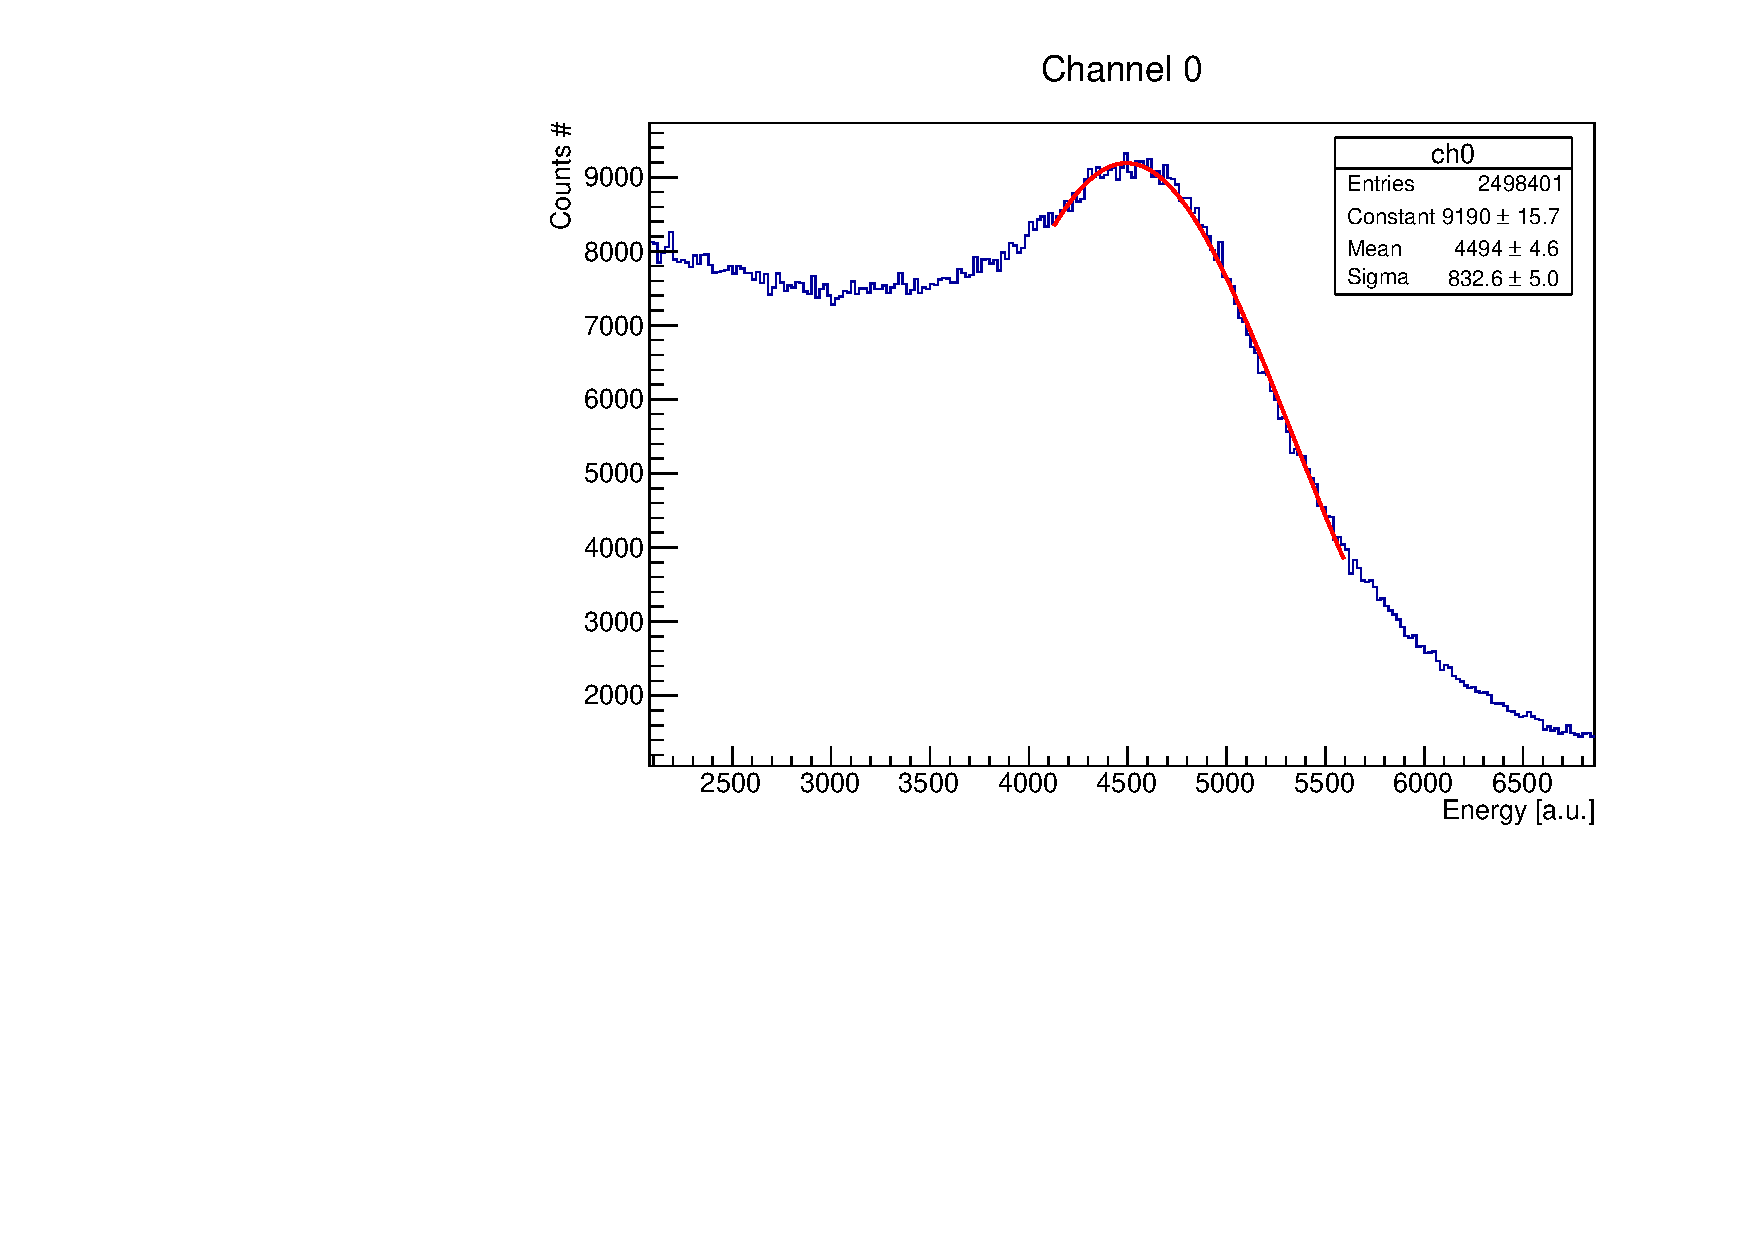
\includegraphics[width=.45\textwidth]{fit_511_d1}} \quad
\subfloat[][\emph{High energy Compton Edge}.]
   {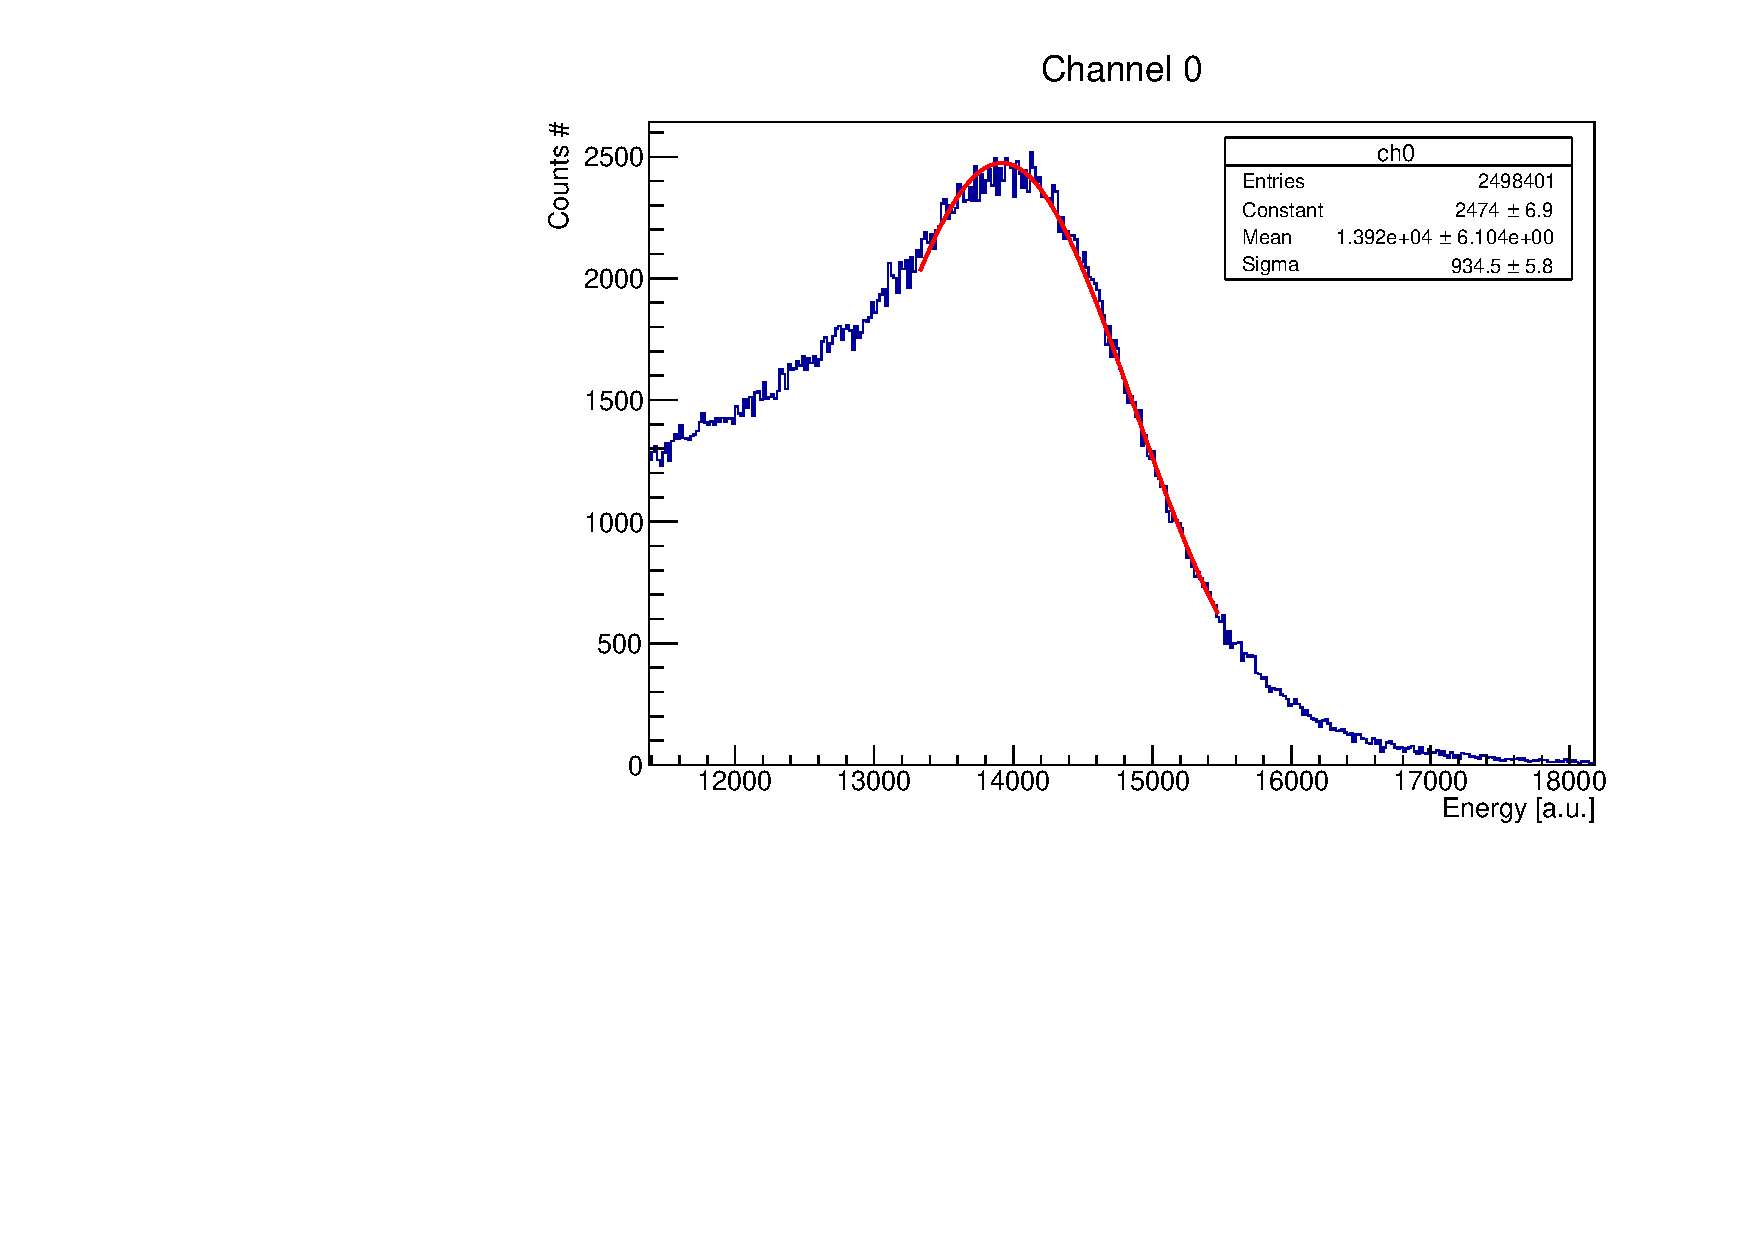
\includegraphics[width=.45\textwidth]{fit_1275_d1}} \\
\caption{Compton Edge for Detector \#1 .}
\end{figure}

\begin{figure}[h!]
\centering
\subfloat[][\emph{Low energy Compton Edge}.]
   {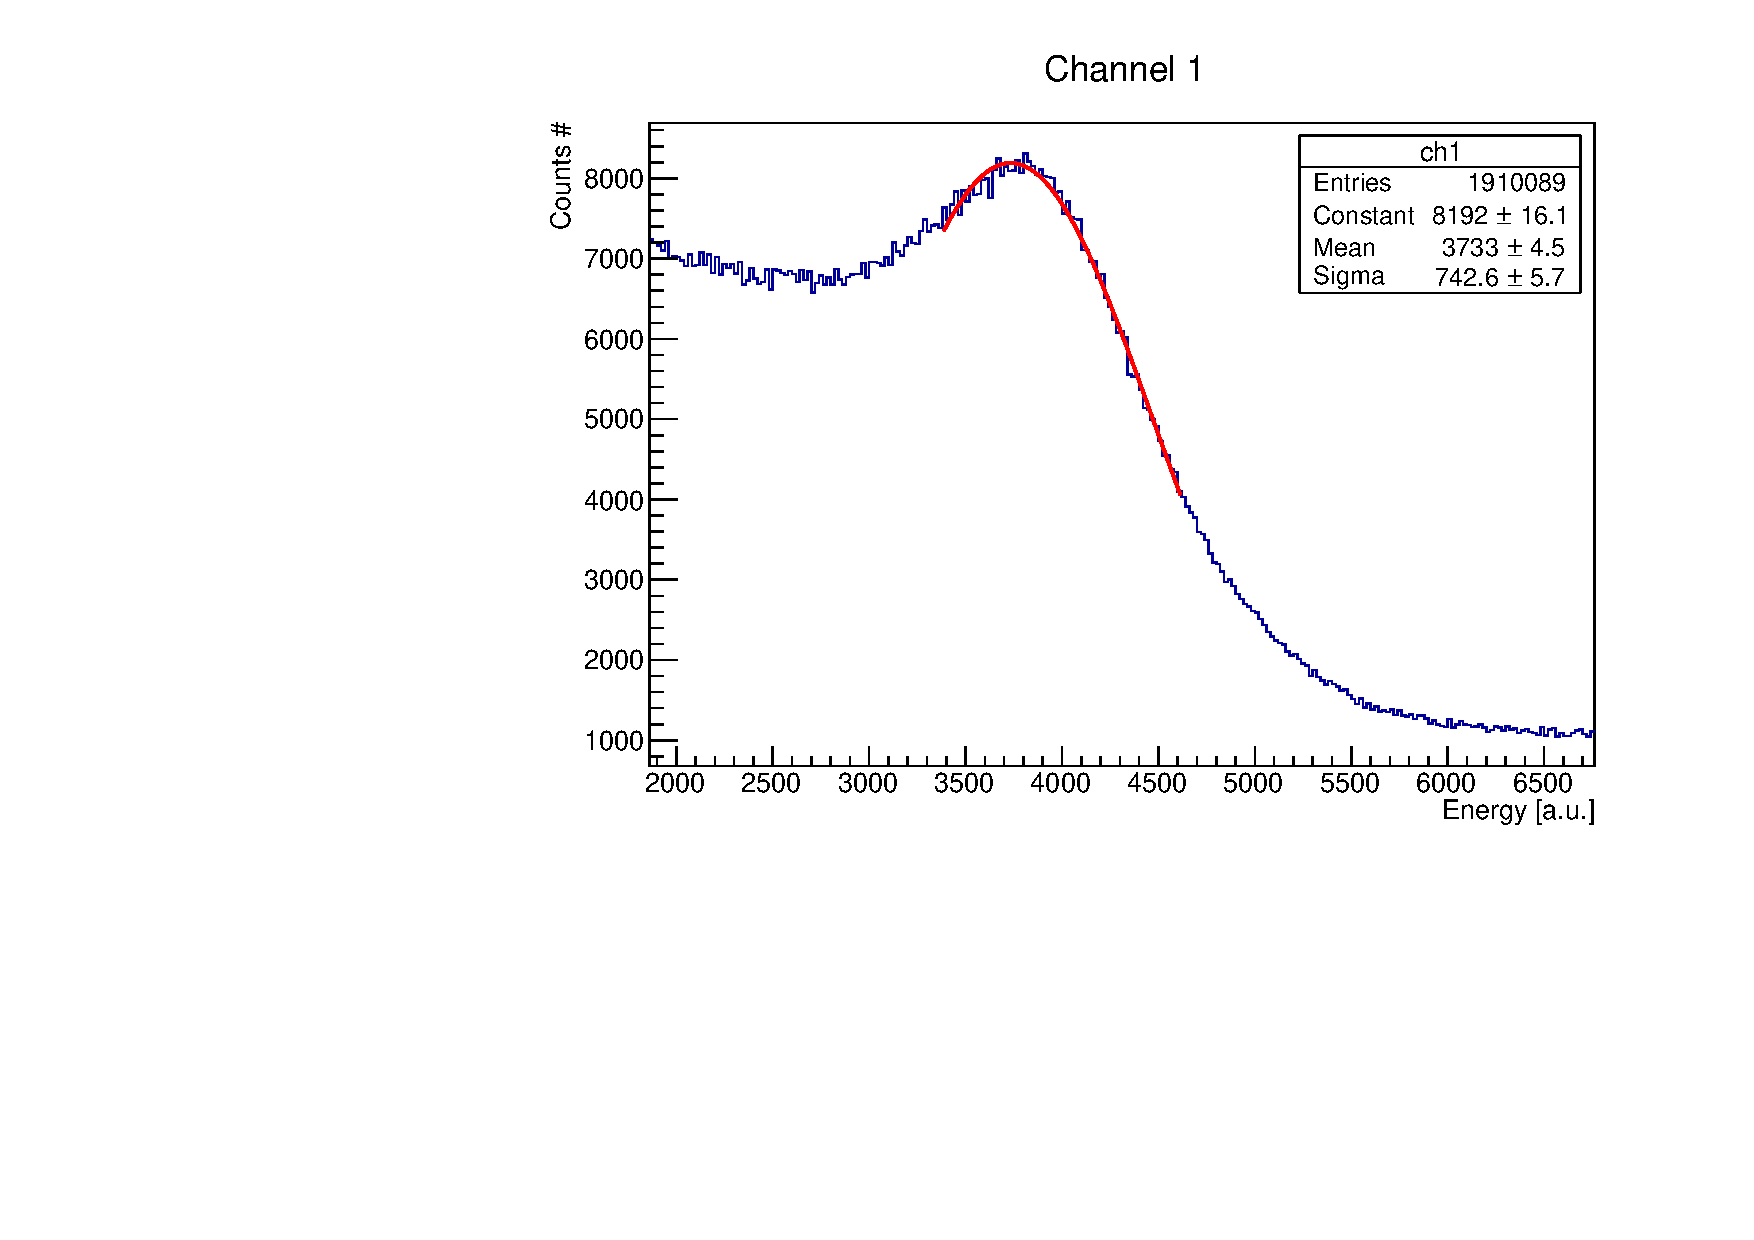
\includegraphics[width=.45\textwidth]{fit_511_d2}} \quad
\subfloat[][\emph{High energy Compton Edge}.]
   {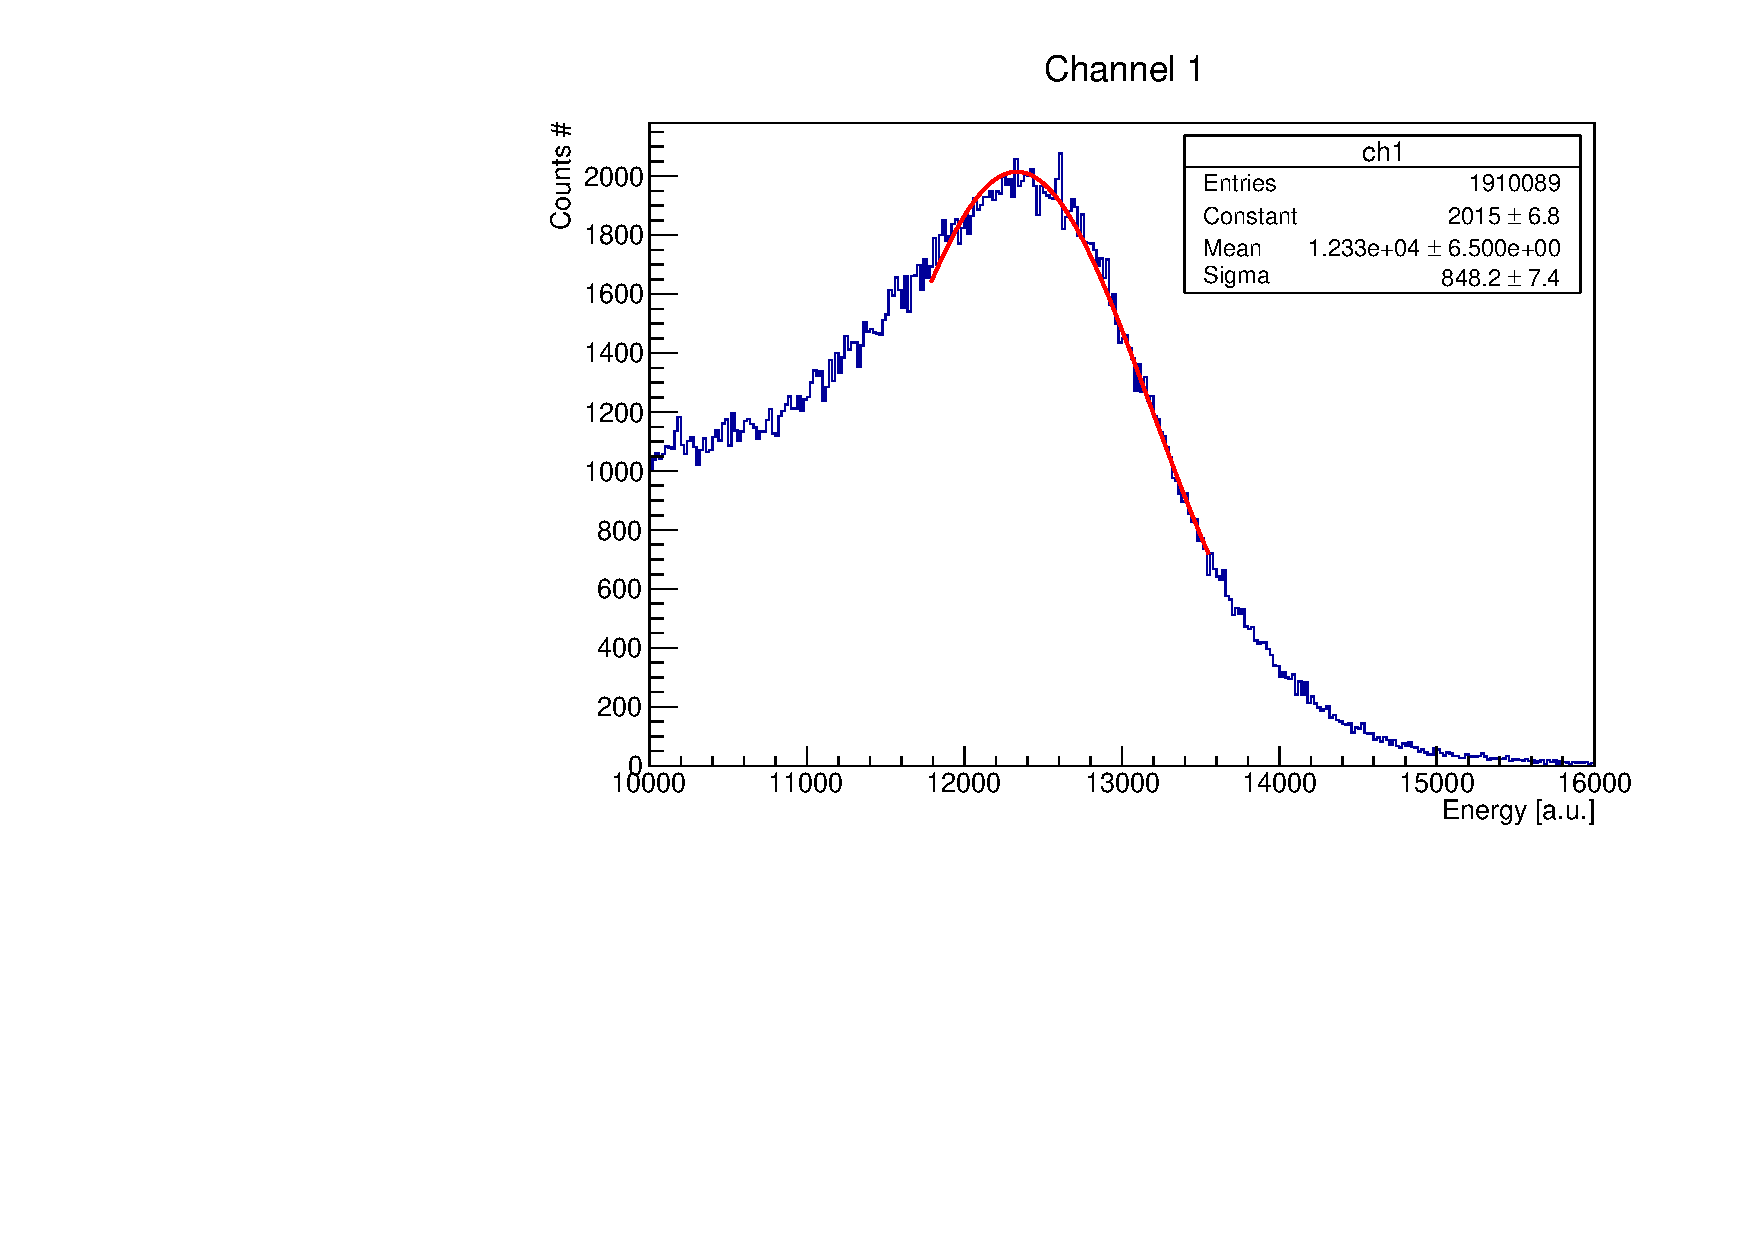
\includegraphics[width=.45\textwidth]{fit_1275_d2}} \\
\caption{Compton Edge for Detector \#2 .}
\end{figure}

\clearpage
\section*{TAC calibration}
In order to calibrate the TAC we have acquired data using auto coincidence between a detector signal and itself. By changing the delay in the delay unit we have obtained the spectra in the Fig. \ref{fig: uncalibrated TAC}. Then using TSpectrum we have found the peaks centroid and fit the using a linear function (Fig. \ref{fig: fit tac}). The calibrated spectra is shown in Fig. \ref{fig: calibrated TAC}.
\begin{figure}[h!]
\centering
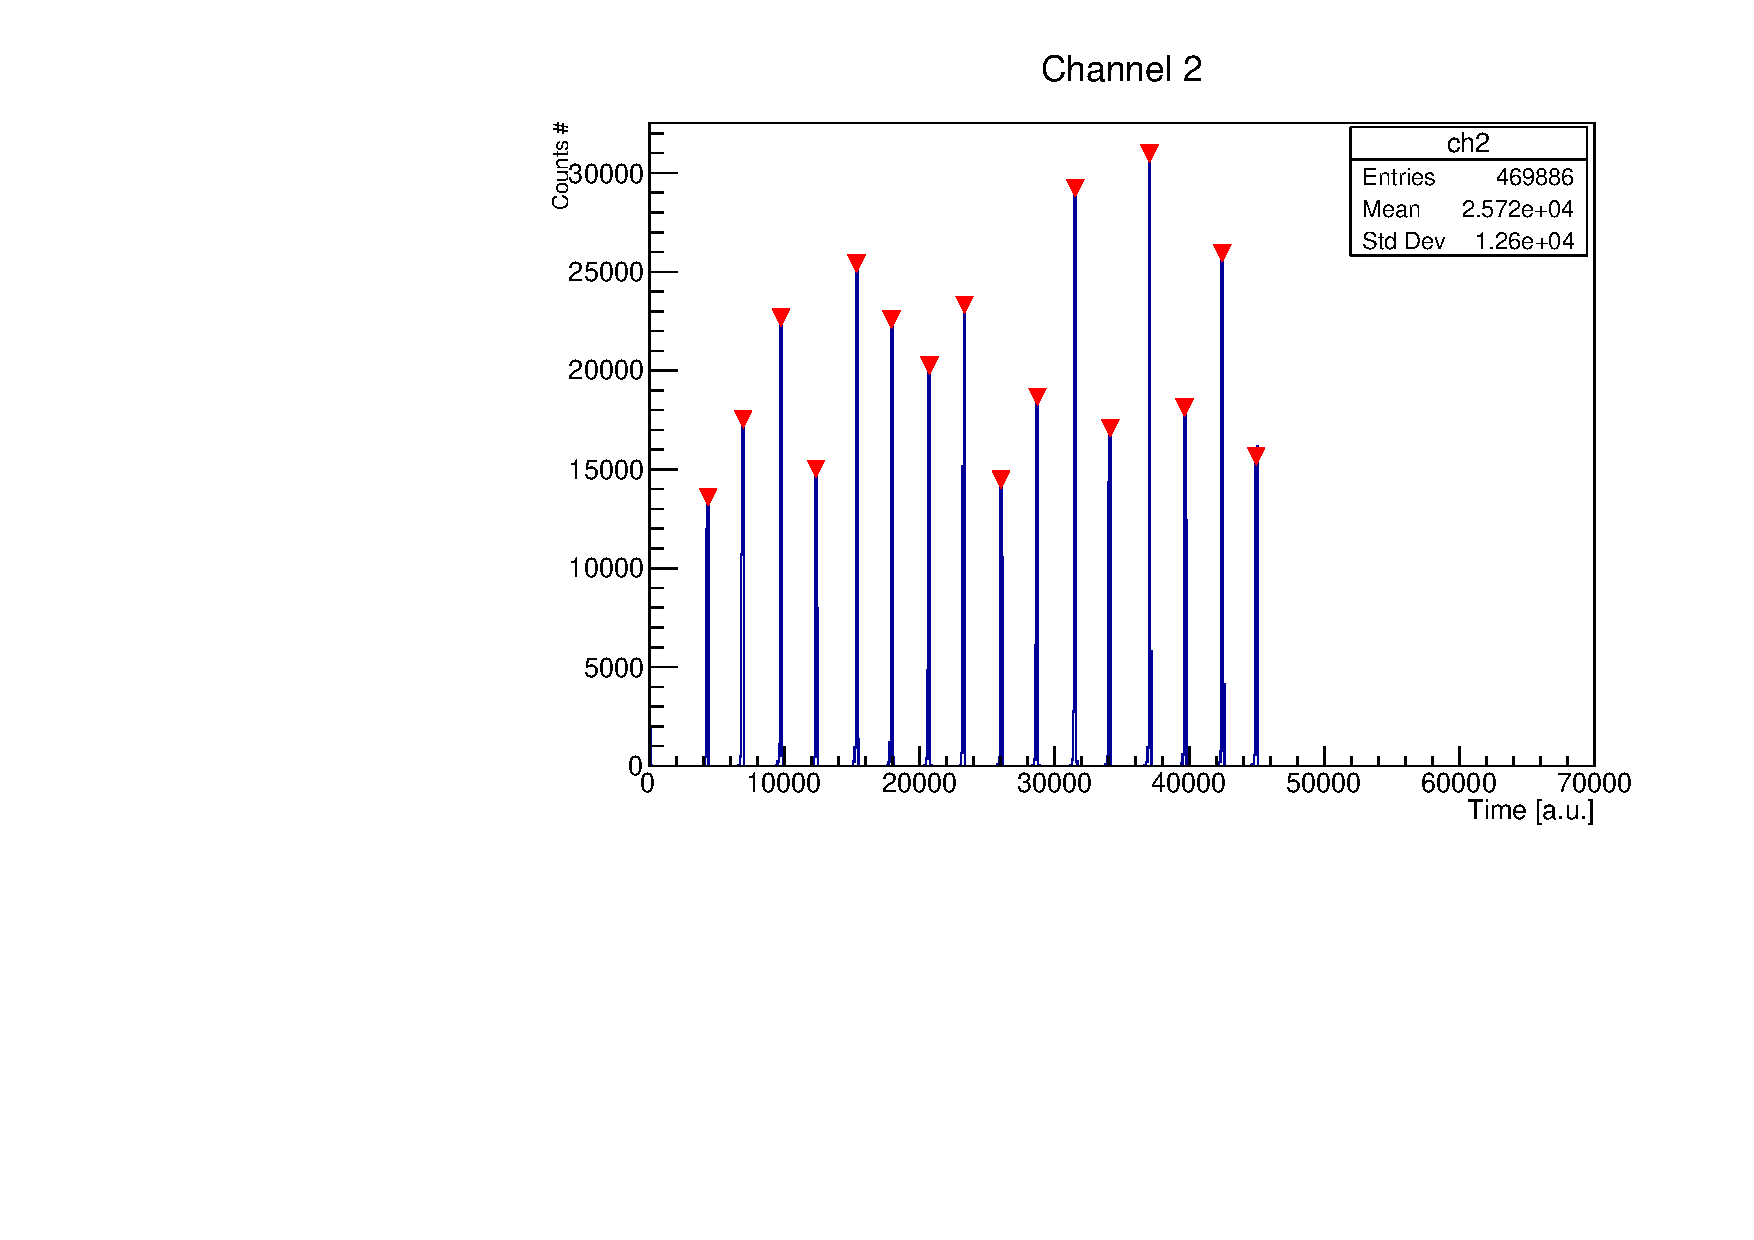
\includegraphics[width=\textwidth]{tac_uncalibrated_spectrum.pdf}
\caption{TAC spectrum (not calibrated). Obtained with an autocoincidence.}
\label{fig: uncalibrated TAC}
\end{figure}


\begin{figure}[h!]
\begin{minipage}[b]{0.6\textwidth}
\centering
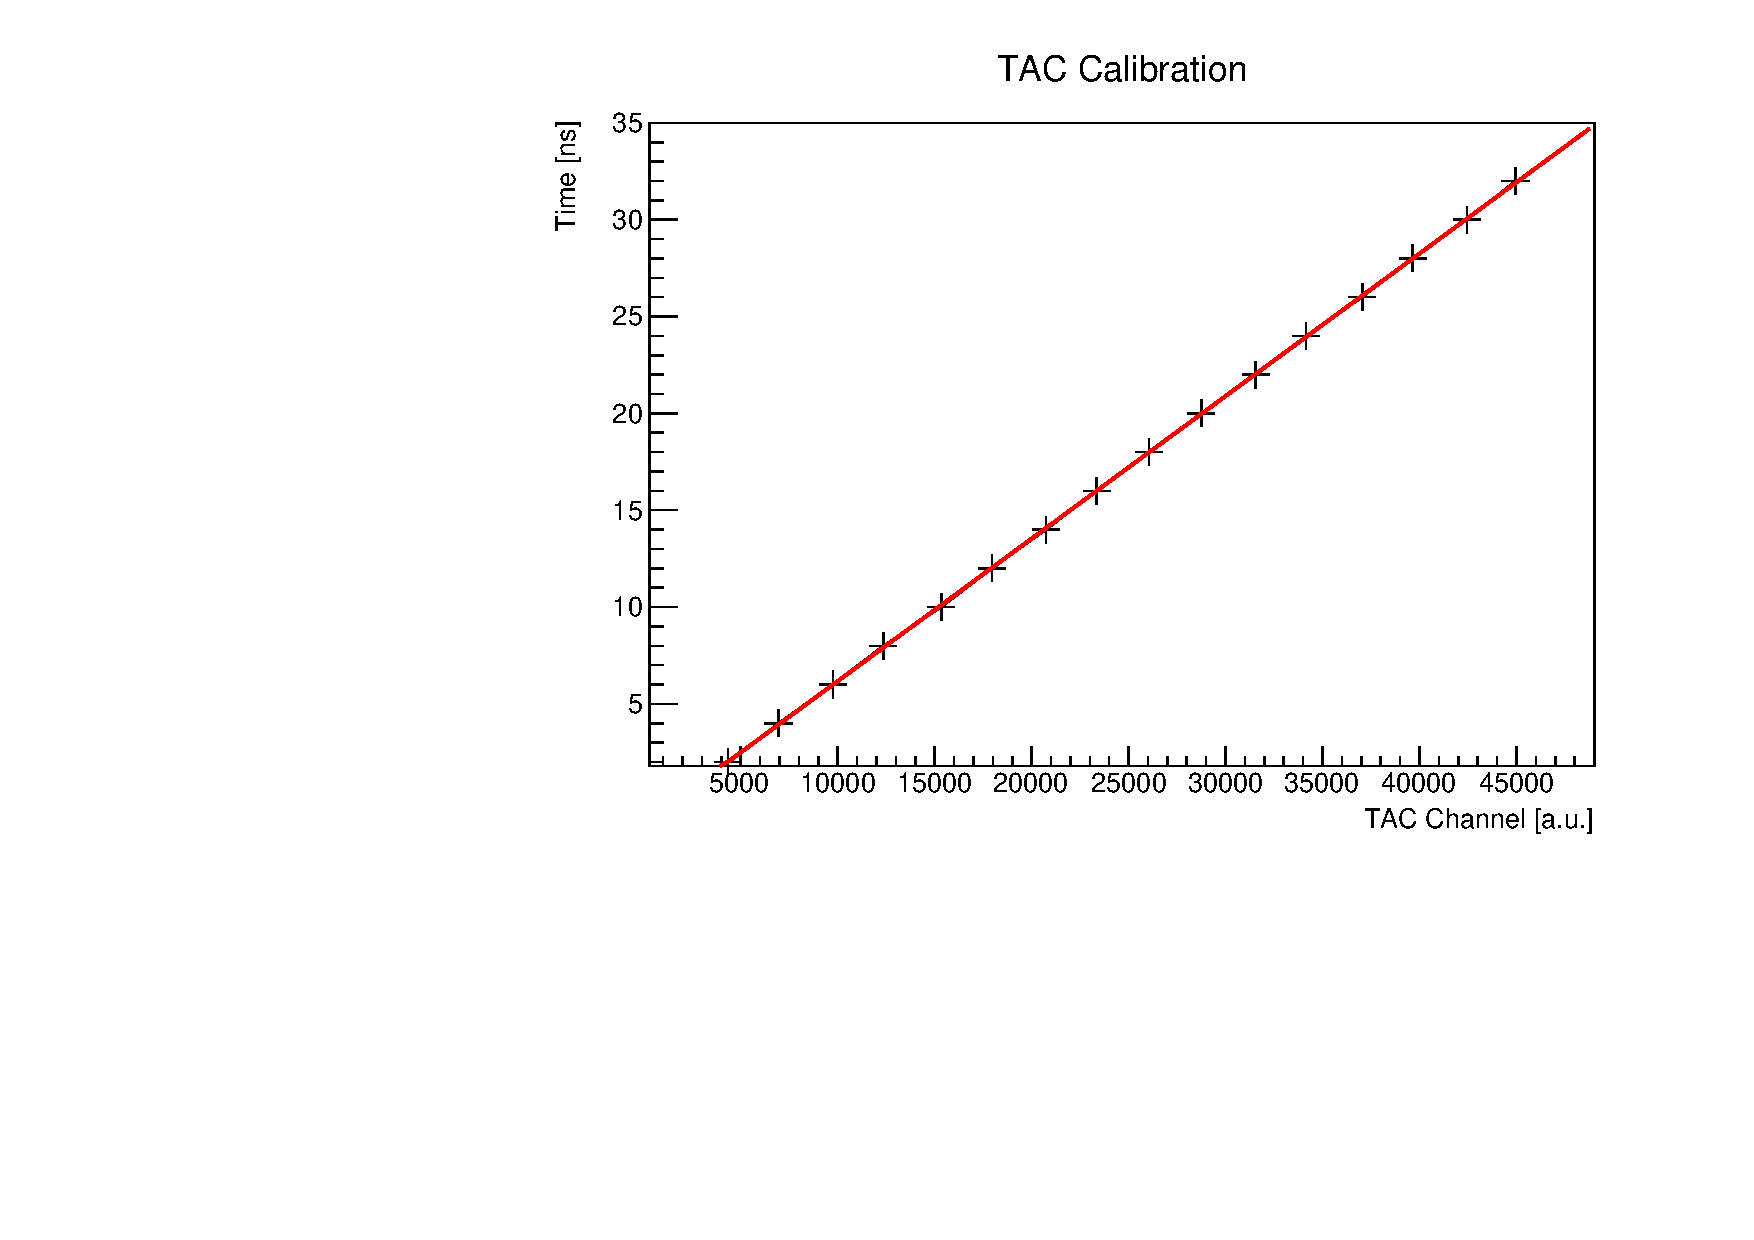
\includegraphics[width=\textwidth]{fit_calibrazione_tac}
\caption{Fit for TAC calibration.}
\label{fig: fit tac}
\end{minipage}
\hfill
\begin{minipage}[b]{0.45\textwidth}
\centering
\begin{tabular}{cc}
\toprule
\toprule
Parameter & Value \\
\midrule
p0     & -1.19 $\pm$  0.04 \\
p1     &  0.000736   $\pm$  0.000001\\
\bottomrule
\bottomrule
\end{tabular}
\vspace{1.5cm}
\caption{Fit parameters.}
\end{minipage}

\end{figure}

\begin{figure}[h!]
\centering
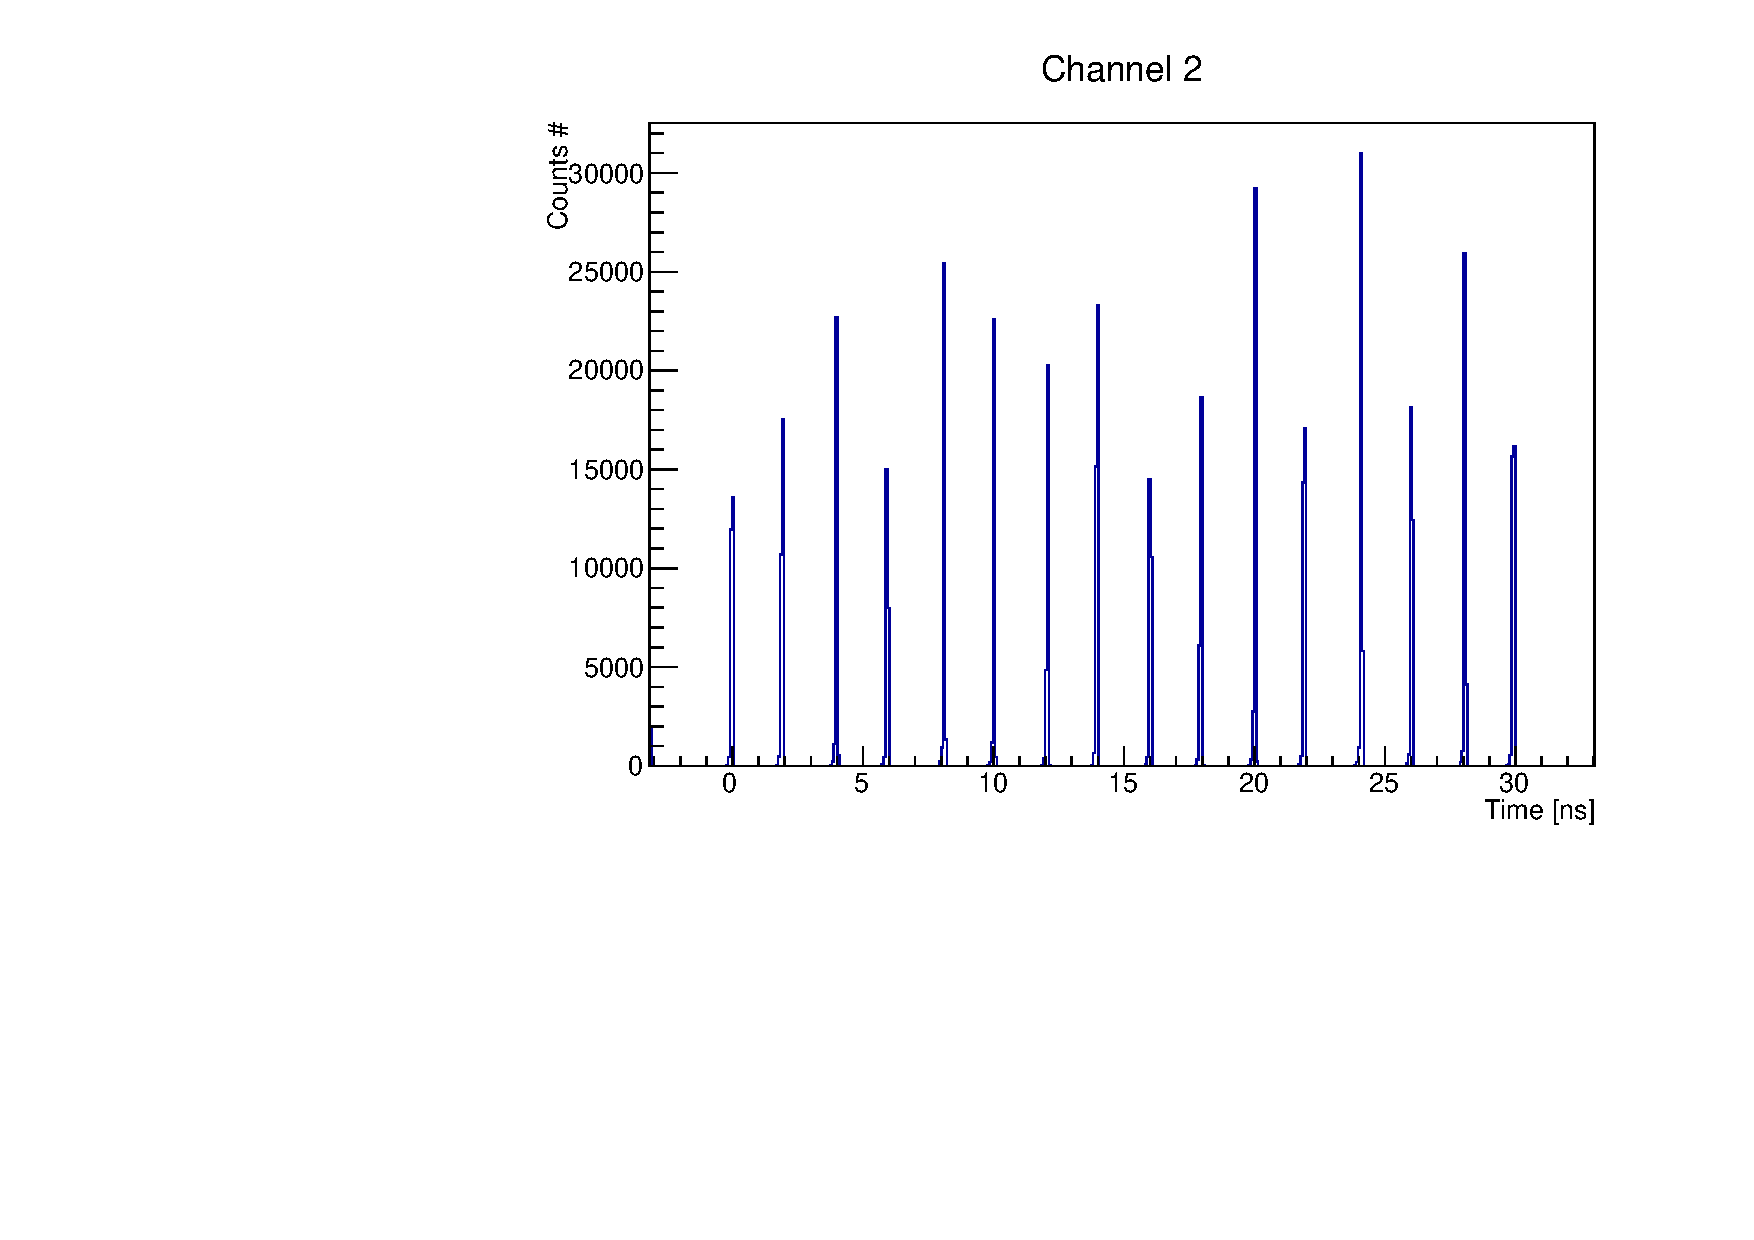
\includegraphics[width=\textwidth]{tac_calibrato}
\caption{Calibrated TAC spectrum. }
\label{fig: calibrated TAC}
\end{figure}
\clearpage
\section{External delay optimization}

\begin{figure}[h!]
\centering
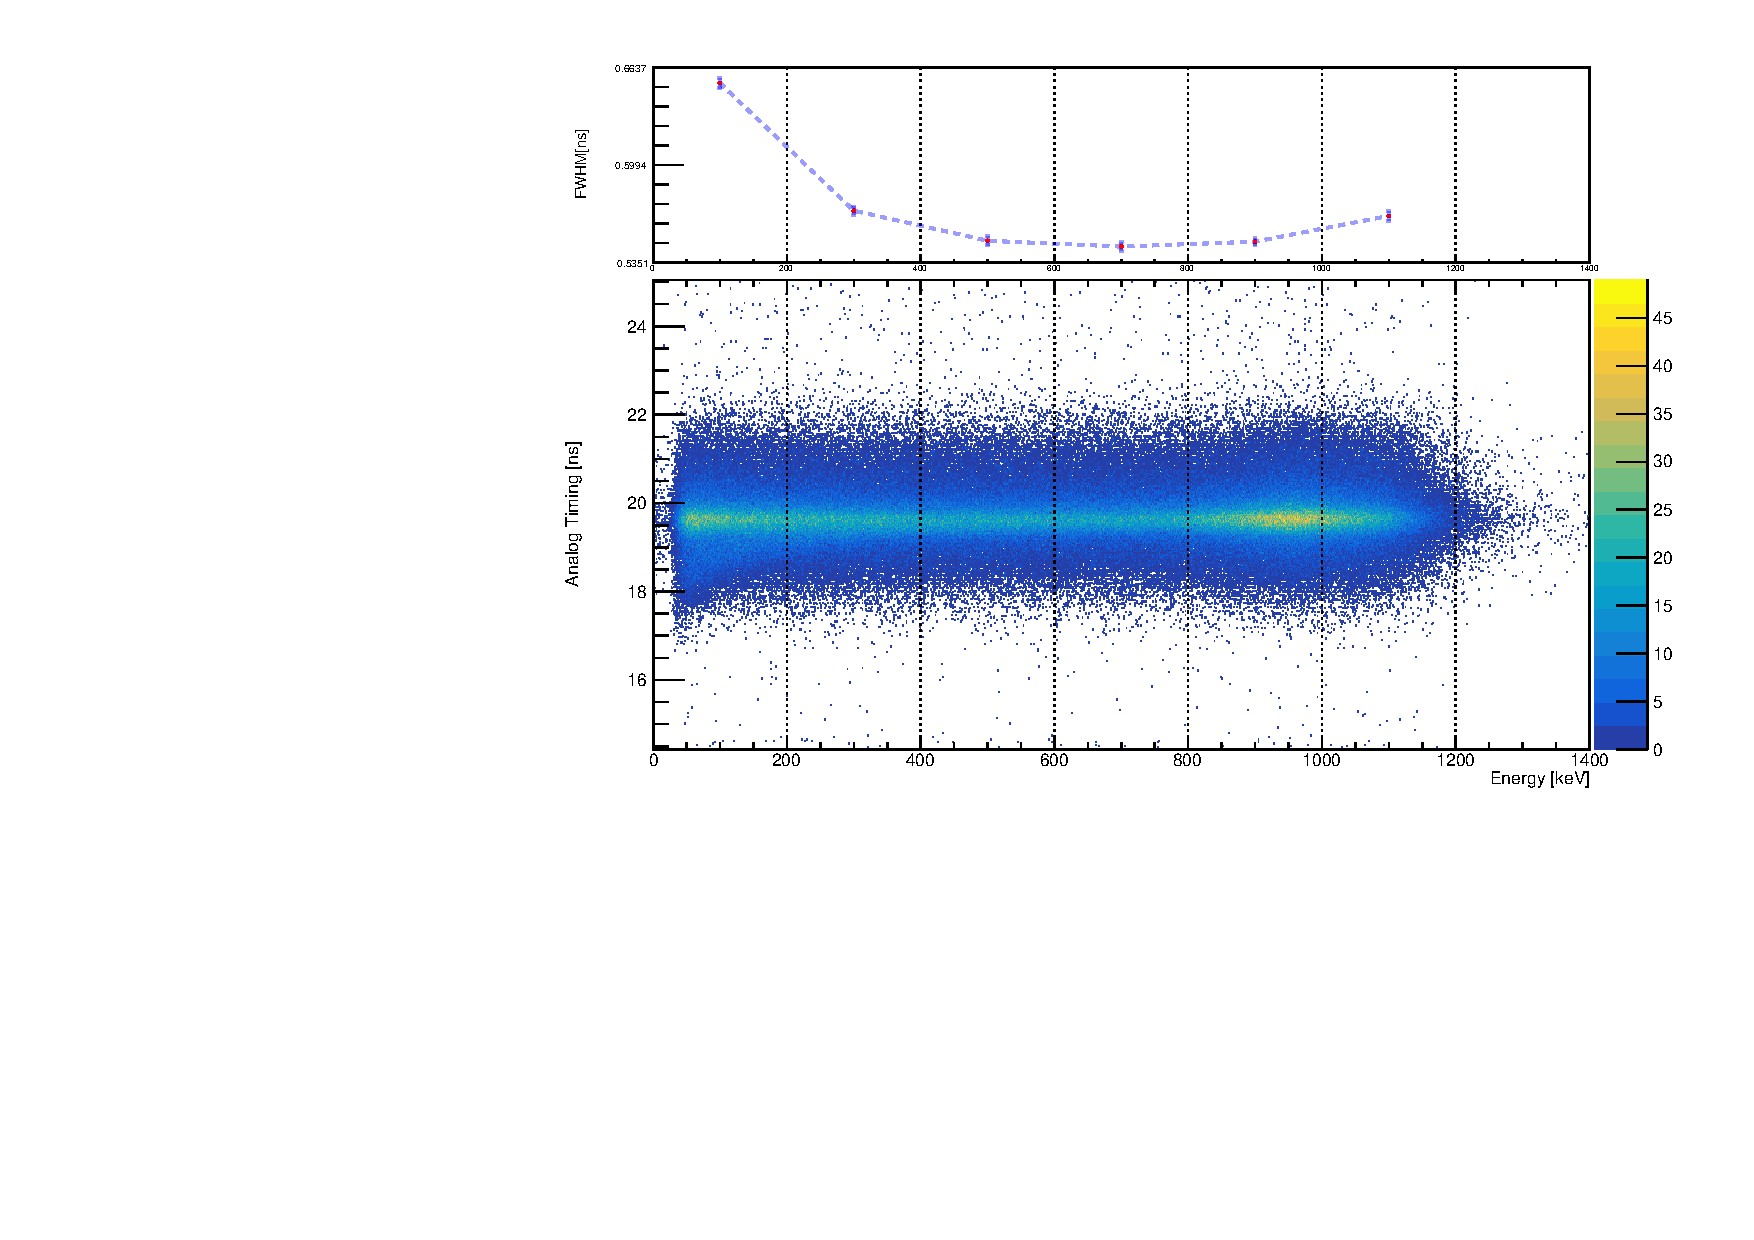
\includegraphics[width=\textwidth]{grafico_editato}
\caption{Dynamic Range.}
\end{figure}






\end{document}
